\documentclass[10pt,a4paper,oneside]{article}
\usepackage{amsmath,amsthm,amssymb,floatrow}
\usepackage{lmodern}
\usepackage{geometry}
\usepackage{graphicx,float,subfigure,ctex}
\DeclareGraphicsExtensions{.pdf,.jpeg,.png,.jpg}
\geometry{left=2.18cm,right=2.18cm,top=1.54cm,bottom=2.0cm}
\pagestyle{empty}
\title{\bf 2024秋数值代数--实验报告 \#1}
\author{姓名:李奕萱  学号:PB22000161 }
\date{\today}

\begin{document}

%\title{\huge{\textbf{2023秋计算方法-实验报告\#1}}}
%\author{姓名:\underline{   }\hspace{1cm}学号:PB2151xxxx}
\maketitle

运行环境:[win11,vscode,py3]
%win11,vscode,py3

\section*{实验内容与要求}
\begin{itemize}
  \item{问题1:}
  给定两个函数~$\color{blue}f(x)=\sqrt{x^2+25}-5$~和~$\color{blue}g(x)=\frac{x^2}{\sqrt{x^2+25}+5}$,
{\bf\color{red} 采用单精度}(即float型)进行编程~(注意:开方sqrt(x)等内置函数的输出结果默认是双精度,
需要强制转成单精度), 分别取
~$\color{blue}x=4^{-1}, 4^{-2}, 4^{-3}, \cdots, 4^{-11}$,
输出相应的函数值~$\color{blue}f(x)$~和~$\color{blue}g(x)$,
计算结果{\bf 保留12位尾数}(用科学计数形式, 参见表1中的数据格式),比较并分析两种方法得到的计算结果。
你认为哪种方法得到的计算结果更可靠?请给出你的理由或分析。

  \item{问题2:} 给定如下数据
 
%%4042.045051380452, 0.000531415926535, -2759471.276702747, -34.64291531266504, \\
%%2755463.874010974, -0.000031415926535, 0.0000557052996742893.每一步的计算结果,

4042.045051380452, 0.000531415926535, -2759471.276702747, 0.0000557052996742895, \\
2755463.874010974, -34.64291531256604,  -0.000031415926535.

分别采取以下4种方式求和:

(a) 顺序求和; ~~~~(b) 逆序(从后往前)求和;

(c) 按绝对值从大到小的顺序, 依次求和;
%正数从大到小依次求和,负数从小到大依次求和,然后二者相加;

(d) 按绝对值从小到大的顺序, 依次求和.
%正数从小到大依次求和,负数从大到小依次求和,然后二者相加.

采{\bf\color{red} 用双精度}进行计算,计算结果中的尾数至少保留9位小数(用科学计数形式,比如1.234567899E$-11$). 
比较4种方法得到的计算结果;你认为哪种方法得到的计算结果更精确(即误差最小;提示:想办法算出精确值)?
试给出你的理由或分析。


\item{问题3:~(计算结果保留10位有效数字)}  Let $\pi \approx 3.14159 26535 897932.$ 
%=3.14159265358979323846264338327950
%$\frac{\pi}{2024}, \frac{\pi}{10}, \frac{\pi}{6}, \frac{\pi}{4}, \frac{\pi}{3}$
\vspace{-0.1in}
\begin{figure}[htb]% 插入两张图片并且并排
	\centering
    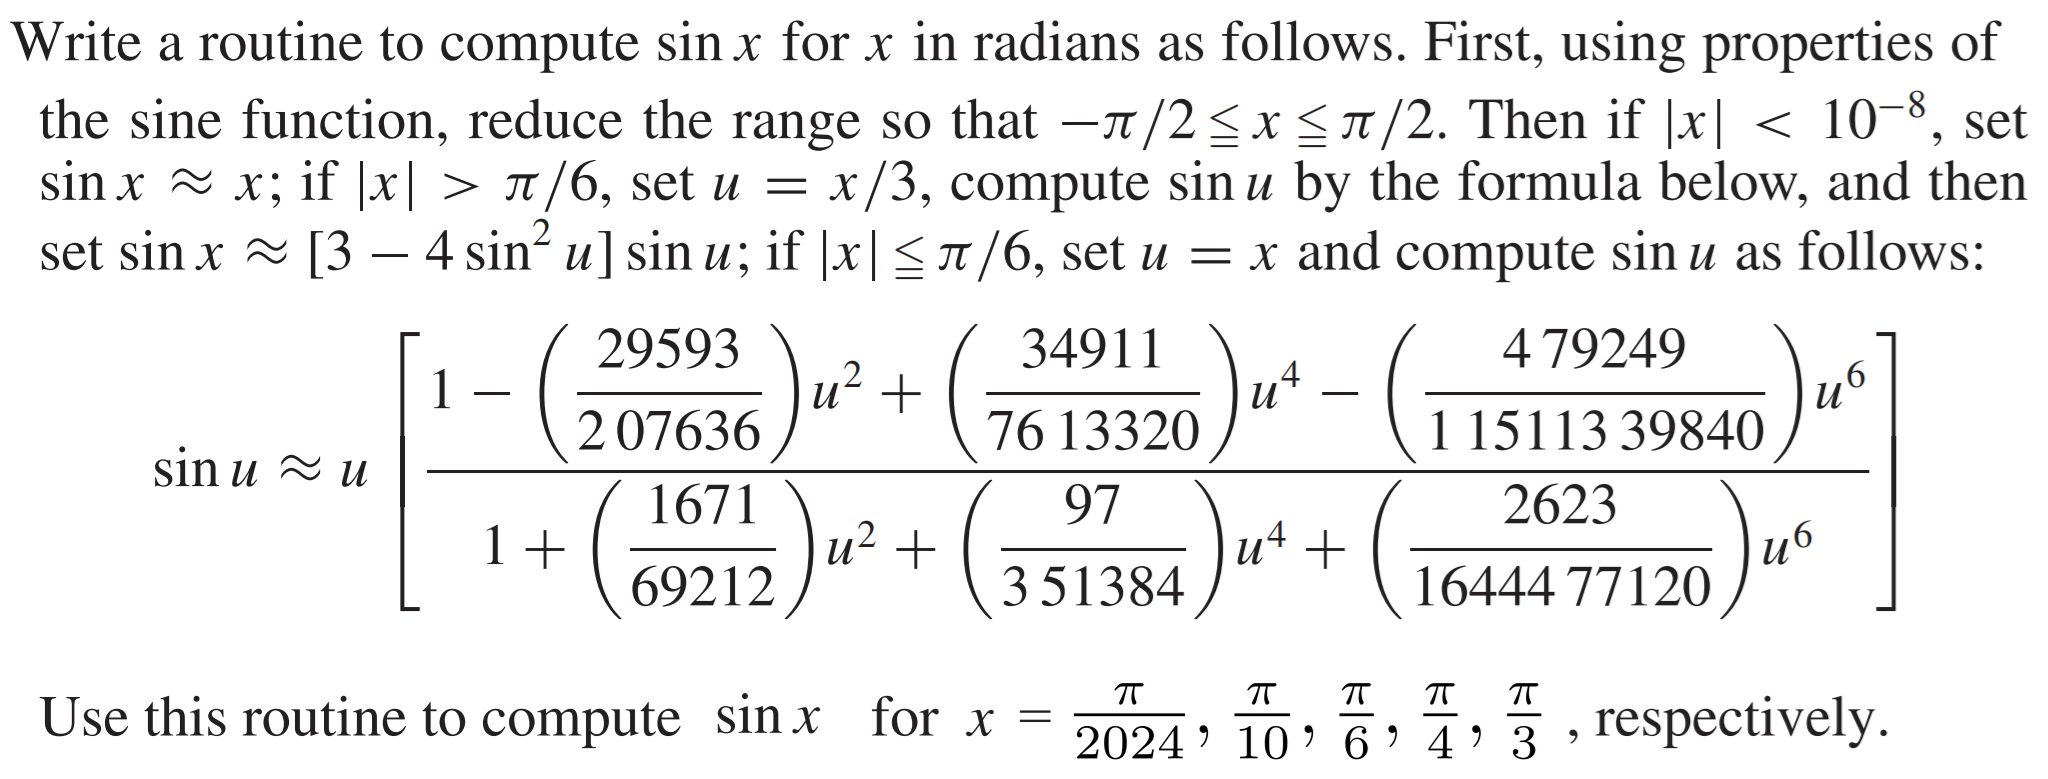
\includegraphics[width=5.40in]{lab01c(1).png}
  %\caption{\fontsize{9pt}{0pt} N=4 (Left), N=8 (Right)}
\end{figure}

\vspace{-0.2in}
Compare those results with results obtained by the Taylor formula, i.e., $\sin(x) \approx x- \frac{x^3}{3!} +  \frac{x^5}{5!} - \frac{x^7}{7!}$.
\end{itemize}

\clearpage

\section{数值结果(请尽量列表或作图)}
\begin{itemize}
  \item 问题1
\begin{figure}[H]
  \centering
  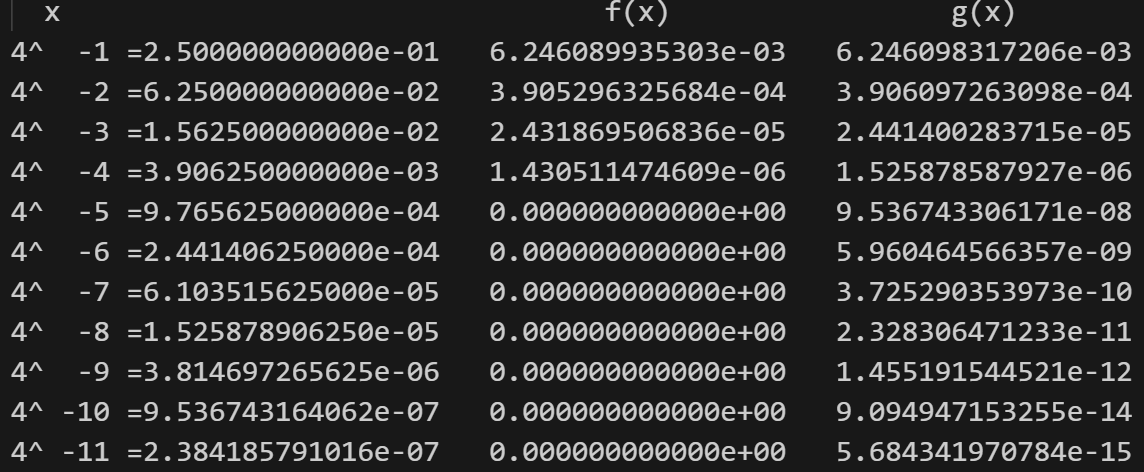
\includegraphics[width=0.9\textwidth]{屏幕截图 2024-09-12 184759.png} 
  \caption{题1计算结果}
\end{figure}

\item  问题2~(用科学计数形式, 尾数至少保留9位小数)

\begin{figure}[H]
  \centering
  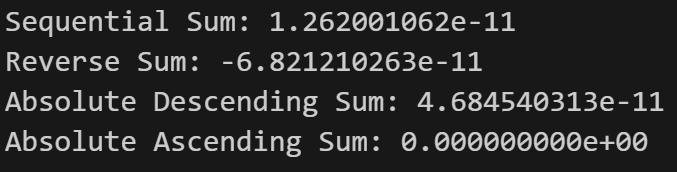
\includegraphics[width=0.9\textwidth]{屏幕截图 2024-09-06 223952.png}
  \caption{题2计算结果(mathematica精确计算结果同第三个)}
\end{figure}


 \item  问题3~(保留10位有效数字, $\pi \approx 3.14159 26535 897932$)
 \begin{figure}[H]
  \centering
  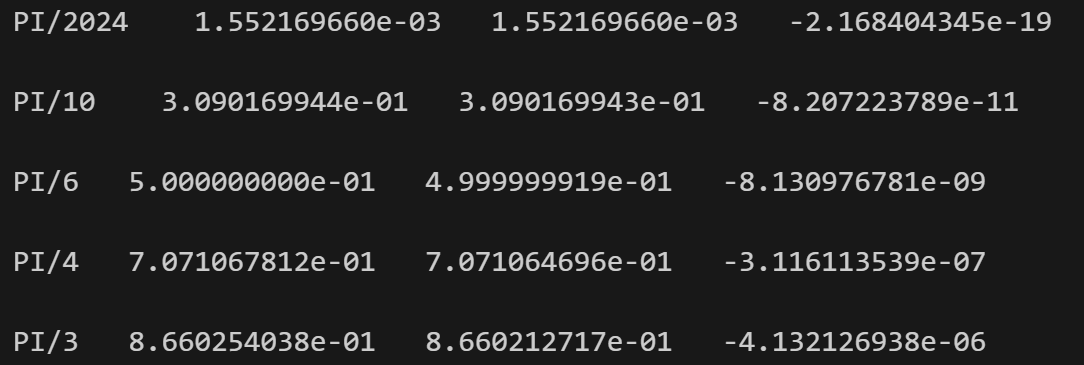
\includegraphics[width=0.8\textwidth]{屏幕截图 2024-09-07 133238.png}
  \caption{题3计算结果(其中第二列是题给方法,第三列是Taylor展开方法,最右边为二者之差)}
\end{figure}
 
 %$\frac{\pi}{2024}, \frac{\pi}{10}, \frac{\pi}{6}, \frac{\pi}{4}, \frac{\pi}{3}$

\end{itemize}


\section{算法分析}
\begin{itemize}
  \item 问题1
  
  Step1:分别定义$f(x)$和$g(x)$,注意控制精度。

  Step2:构建循环输出结果。
  
  \item 问题2
  
  Step1:输入数据

  Step2:分别定义四种求和(注意控制精度)

  step3:输出四种求和的结果

  \item 问题3
  
  Step1:定义题目中的函数

  Step2:定义Taylor函数

  step3:分别输出二者结果并进行比较

\end{itemize}


\section{结果分析}

\begin{itemize}
  \item 问题一
  $f(x)$和$g(x)$为同一算式的不同表达方式
  
  二者计算误差如下:
  \begin{figure}[H]
    \centering
    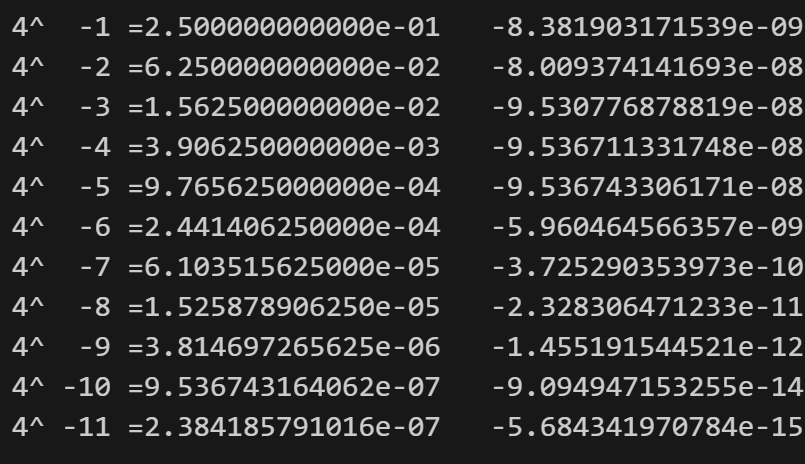
\includegraphics[width=0.7\textwidth]{屏幕截图 2024-09-12 184815.png}
    \caption{f(x)和g(x)误差如下}
  \end{figure}
  我认为$f(x)$计算结果更可靠,math.sqrt这一步结果为双精度,当强行切换为单精度
  时,会产生舍入误差,除法亦是同理,误差积累,所以我认为$f(x)$结果更可靠。
  
  \begin{figure}[H]
    \centering
    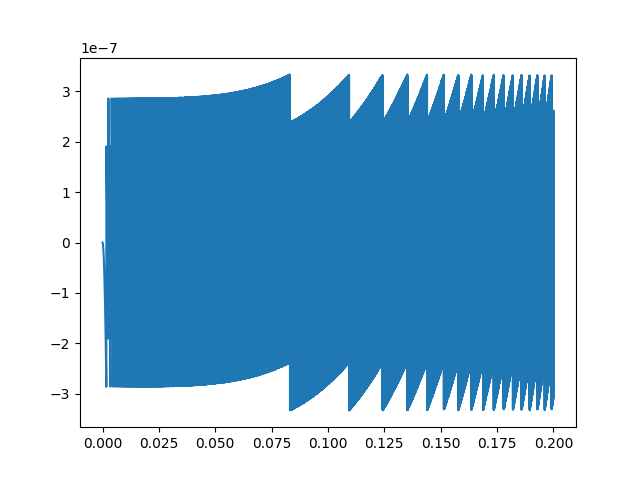
\includegraphics[width=0.7\textwidth]{Figure_1.png}
    \caption{f(x)和g(x)误差作图(步长为1e-7)}
  \end{figure}

  同时可以发现,当数字较大的时候(对应步长较大),二者相对误差接近0,
  ,当逐渐减小时(对应步长减小),误差会突然增大,然后再逐渐降低。

  \item 问题二
  
  在与精确结果进行对比后得知,第三种方法得到的结果最精确,进分析,
绝对值较大的数可存储的小数点后的位数最少,而绝对值较小的数则可储存较多,
由此可见,按绝对值从大到小的顺序进行计算可以尽可能地保留小数点后面的精度。
  \item 问题三
  \begin{figure}[H]
    \centering
    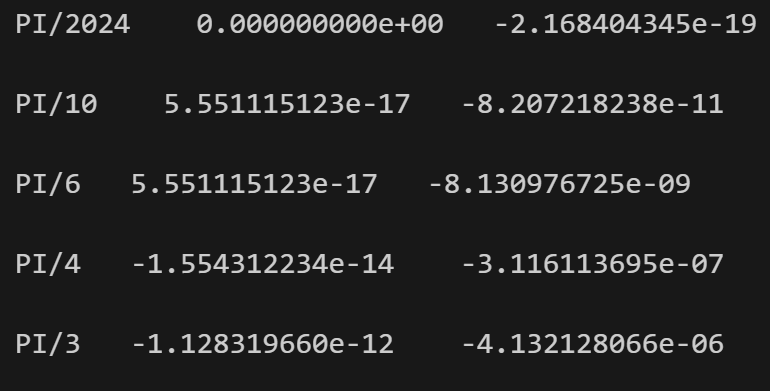
\includegraphics[width=0.8\textwidth]{屏幕截图 2024-09-07 133244.png}
    \caption{两种算法分别和sin的误差值(左边是题目算法,右边是Taylor算法}
  \end{figure}
  从计算结果可以看出,数值越小,二者相对误差越小,同时与标准值进行比较后,
  可以得出,题目给的方法会更加精确。
\end{itemize}


\section{实验小结}

在本次数值实验中,我们分别做了三个小问题,从同一个函数不同表达形式、
不同顺序求和方式、对同一个数值的不同近似表达分别进行了实验,可以得出:

\begin{enumerate}
  \item 对于同一个式子的不同精确表达形式,计算次数少的会更加可靠准确,
  \item 对于不同顺序求和,按绝对值从小到大的顺序更加准确
  \item 对于一个值的不同近似表达式,精确结果也不一样,
\end{enumerate}

\end{document}
